% ==================================================================
%  Filmstrip of the flight -- one sigconf text width, pdfLaTeX
%  Preamble:  \usepackage{tikz}  (graphicx comes with acmart);
%             flight-filmstrip.png on the graphics path
%  Image:     flight-filmstrip.png (8.20 cm wide, 600 dpi), made by
%             cpp2lean sim/figs/render_strobe.py from the same re-flight and
%             camera as flight-strobe.png (copter_lean with the tuned gains,
%             1 m/s figure-eight course, 400 Hz control, 1200 Hz physics; its
%             actuator lines equal the recorded ones, 0 differ): six
%             instants, each tile the full view with the path flown so far and the
%             vehicle drawn at 7 times its size, 4x supersampled. The image
%             holds no text; a blank strip under the tiles carries the time
%             labels, placed at the tile centers written by the script to
%             sim/figs/out/strobe/film-labels.txt.
% ==================================================================
\definecolor{fwInk}{HTML}{22252A}%
\definecolor{fwMute}{HTML}{8A8F96}%
\begin{tikzpicture}[fl/.style={font=\footnotesize, text=fwMute, inner sep=0pt, anchor=mid}]
\node[anchor=south west, inner sep=0] (img) at (0,0)
  {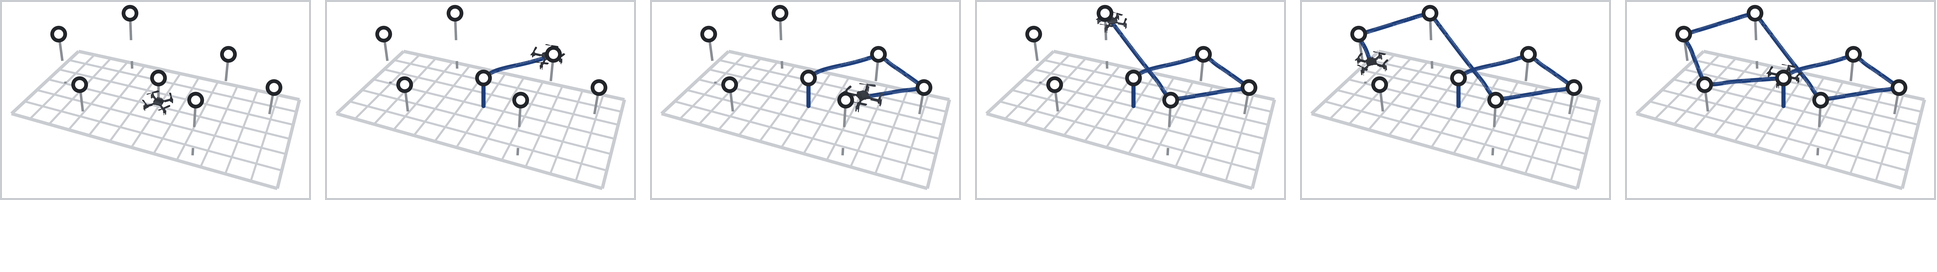
\includegraphics[width=\linewidth]{flight-filmstrip.png}};
\begin{scope}[x={(img.south east)}, y={(img.north west)}]
  \node[fl] at (0.0803,0.1324) {$t=0$\,s};
  \node[fl] at (0.2481,0.1324) {3.5\,s};
  \node[fl] at (0.4158,0.1324) {7\,s};
  \node[fl] at (0.5836,0.1324) {10.5\,s};
  \node[fl] at (0.7514,0.1324) {14\,s};
  \node[fl] at (0.9192,0.1324) {18.5\,s};
\end{scope}
\end{tikzpicture}%
